
\section{Sending video over network}
Several different methods were tested to provide a livestream of the images taken by the cameras.
Ideally a separate variable bitrate video encoder would be used to encode the images into a video stream and serve it over the network to a video streaming client in a web browser on the phone.
This would allow the user to view the video stream with maximum quality given the available bandwidth.

\subsection{Streaming MP4 videos}
Streaming existing \gls{mp4} video files can easily be done by serving the file over \gls{http} using a simple Python web server and the default video player in \chrome.
Unfortunately it proved more difficult to live stream video in real time.

The first attempt at streaming video in realtime was to serve \gls{mp4} data from \gs as if it was a file and using the \gls{dash} Player to automatically go to the next video segment when the previous one was finished.
This worked to some degree, but requiered a latency of several seconds and had notiable jumps between segments.

The secont approach was done following a blog post from Dusan Kovacevic on how to stream video to a web broser over \gls{hls}, but did not yield a working result \cite{kovacevicStreamLiveVideo2020}.

The third approach was using \gls{rtsp}.
It was however possible to stream video to \gls{vlc} over \gls{rtsp} but it did not work in the web browser.

\subsection{Streaming JPEGs}
As it proved difficult to stream videostreams, the next approach was to stream \glspl{jpeg} over the network instead.
For the current usecase, which is to veryify that the camera is working properly, compression loss or reduced framerate it not viewed as a major problem.
The first attempt was to simply serve image data from a Python web server and ruotinely update the image on the web page.
This worked fine but resulted in a non-smooth framerate as the the same image was sometimes served twice in a row.
To solve this \glspl{ws} were used to serve the images instead.
They made it possible for the server to push data to the client when new images were available, rather than relying on the client polling the server for new data.

\subsubsection{Base64 encoding}
An easy way to serve \glspl{jpeg} is to encode them as base64 strings and serve them as text \cite{rAnswerHowDisplay2013}
Initially this encoding was done serverside but as base64 encoding at least 33\% overhead a small \gls{js} scripted was written to do the encoding clientside instead, shown in Listing \ref{listing:base64}.
It is expeted to possible to update the image from raw \gls{jpeg} bytes, but this was not prioritized as the base64 encoding was easy to implement and worked well enough.
\begin{listing}[H]
    \begin{minted}{js}
        if (message) {
        return message.data.arrayBuffer().then(buffer => {
            let b64 = btoa(String.fromCharCode(...new Uint8Array(buffer)));
            return "data:image/jpeg;base64," + b64; });
        } else {return no_update};
    \end{minted}
    \caption{JavaScript code for encoding \gls{jpeg} data as base64 strings}
    \label{listing:base64}
\end{listing}



\subsection{Future work: Streaming video using WebRTC}
Attempts were also made at integrating an example project from \gs  to stream videos using \gls{webrtc} \cite{gstreamerWebrtcMasterGStreamer2021}.
The example demonstrates the process of streaming video from a pipeline to a client within a web browser. It involves extensive code, consisting of several hundred lines in \py and \gls{js}.
Due to the solution utilizing \glspl{jpeg} had already been implemented, and considering the time-consuming nature of the integration task, it was not given high priority.
In future work acheiving this is probably the best approach as \gls{webrtc} has low latency compared to other protocols as shown in Figure \ref{fig:streaming_latency} \cite{doughertyUltraLowLatency2022}.
\gls{webrtc} is built for low latency peer-to-peer communication over \gls{udp}, supports \gls{h265} encoding and will support \gls{av1} in the future \cite[1]{loretoRealTimeCommunicationWebRTC2014} \cite{ablyWebRTCVsWebSocket2023} \cite{mekyaFirstHEVC2652020}
\cite{red5proKeyReasonsAV12023}
\begin{figure}[H]
    \centering
    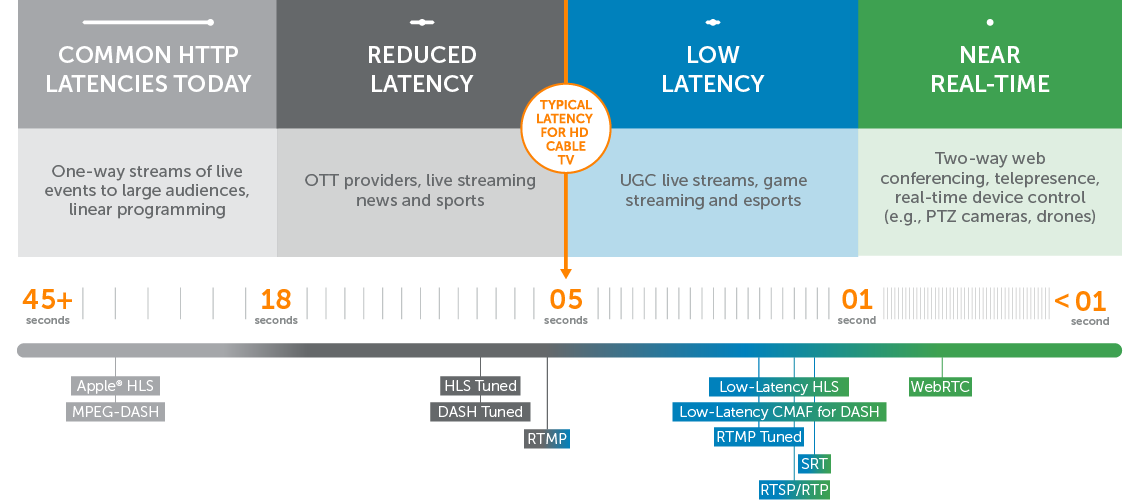
\includegraphics[width=\textwidth]{figures/webrtc_latency.png}
    \caption{Latency comparison of different streaming protocols \cite{doughertyUltraLowLatency2022}}
    \label{fig:streaming_latency}
\end{figure}


